\let\lesson\undefined
\newcommand{\lesson}{\phantomlesson{Bài 17.}}
\setcounter{section}{2}
\section{Trắc nghiệm nhiều phương án lựa chọn}
\setcounter{ex}{0}
\Opensolutionfile{ans}[ans/VN10-2022-PH-TP026-TN]
% ===================================================================
\begin{ex}\mkstar{2}
	Động năng của một vật khối lượng $m$, chuyển động với vận tốc $v$ là
	\choice
	{$W_\text{đ} = \dfrac{1}{2}mv$}
	{\True $W_\text{đ} = \dfrac{1}{2}mv^2$}
	{$W_\text{đ} = mv^2$}
	{$W_\text{đ} = 2mv^2$}
	\loigiai{Động năng của một vật khối lượng $m$, chuyển động với vận tốc $v$ là $W_\text{đ} = \dfrac{1}{2}mv^2$.}
\end{ex}

% ===================================================================
\begin{ex}\mkstar{2}
	Động năng của vật tăng khi
	\choice
	{vận tốc của vật có giá trị âm}
	{vận tốc của vật có giá trị dương}
	{các lực tác dụng lên vật sinh công âm}
	{\True các lực tác dụng lên vật sinh công dương}
	\loigiai{Các lực tác dụng lên vật sinh công dương thì $v$ tăng, do đó động năng tăng.}
\end{ex}
% ===================================================================
\begin{ex}\mkstar{2}
	Độ biến thiên động năng của một vật chuyển động bằng
	\choice
	{công của lực ma sát tác dụng lên vật}
	{công của các lực thế (ví dụ: trọng lực, lực đàn hồi, \dots) tác dụng lên vật}
	{công của trọng lực tác dụng lên vật}
	{\True công của các lực tác dụng lên vật}
	\loigiai{Độ biến thiên động năng của một vật chuyển động bằng công của các lực tác dụng lên vật.}
\end{ex}
% ===================================================================
\begin{ex}\mkstar{2}
	Dạng năng lượng tương tác giữa Trái Đất và vật là	
	\choice
	{động năng}
	{\True thế năng trọng trường}
	{thế năng đàn hồi}
	{cơ năng.}
	\loigiai{Dạng năng lượng tương tác giữa Trái Đất và vật là thế năng trọng trường.}
\end{ex}
% ===================================================================
\begin{ex}\mkstar{2}
	Thế năng trọng trường của một vật
	\choice
	{luôn dương vì độ cao của vật luôn dương}
	{\True có thể âm, dương hoặc bằng không}
	{không thay đổi nếu vật chuyển động thẳng đều}
	{không phụ thuộc vào vị trí của vật}
	\loigiai{	Thế năng trọng trường của một vật có thể âm, dương hoặc bằng không.}
\end{ex}
% ===================================================================
\begin{ex}\mkstar{2}
		Đơn vị nào \textbf{không} phải đơn vị của động năng?
	\choice
	{$\si{\joule}$}
	{\True $\si{\newton/\meter^2}$}
	{$\si{\newton\cdot\meter}$}
	{$\si{\kilogram\cdot\meter^2/\second^2}$}
	\loigiai{}
\end{ex}
% ===================================================================
\begin{ex}\mkstar{2}
	Động năng là đại lượng
	\choice
	{vô hướng, dương, âm hoặc bằng không}
	{\True vô hướng, có thể dương hoặc bằng không}
	{vectơ, luôn dương}
	{vectơ, có thể dương hoặc bằng không}
	\loigiai{}
\end{ex}
% ===================================================================
\begin{ex}\mkstar{2}
Một vật đang chuyển động với vận tốc $v$. Nếu hợp lực tác dụng vào vật triệt tiêu thì động năng của vật	
	\choice
	{giảm theo thời gian}
	{\True không thay đổi}
	{tăng theo thời gian}
	{triệt tiêu}
	\loigiai{}
\end{ex}
% ===================================================================
\begin{ex}\mkstar{2}
	Một vật được ném thẳng đứng từ dưới lên cao. Trong quá trình chuyển động của vật thì
	\choice
	{Thế năng của vật giảm, trọng lực sinh công dương}
	{Thế năng của vật giảm, trọng lực sinh công âm}
	{Thế năng của vật tăng, trọng lực sinh công dương}
	{\True Thế năng của vật tăng, trọng lực sinh công âm}
	\loigiai{Khi một vật được ném lên, độ cao của vật tăng dần nên thế năng tăng.\\
		Trong quá trình chuyển động của vật từ dưới lên, trọng lực luôn hướng ngược chiều chuyển động nên nó là lực cản, do đó trọng lực sinh công âm.}
\end{ex}
% ===================================================================
\begin{ex}\mkstar{2}
	Thế năng trọng trường là đại lượng	
	\choice
	{vô hướng, có thể dương hoặc bằng không}
	{\True vô hướng, có thể âm, dương hoặc bằng không}
	{vector cùng hướng với vector trọng lực}
	{vector có độ lớn luôn dương hoặc bằng không}
	\loigiai{Ta có, thế năng hấp dẫn là đại lượng vô hướng, có thể âm, dương hoặc bằng 0.}
\end{ex}
% ===================================================================
\begin{ex}\mkstar{2}
	Một vật có khối lượng $\SI{250}{g}$ đang di chuyển với tốc độ $\SI{10}{m/s}$. Động năng của vật này là
	\choice
	{\True $\SI{12.5}{\joule}$}
	{$\SI{25}{\joule}$}
	{$\SI{12500}{\joule}$}
	{$\SI{25000}{\joule}$}
	\loigiai{Động năng của vật:
		$$W_\text{đ} = \dfrac{1}{2} mv^2  =\SI{12.5}{J}.$$}
\end{ex}
% ===================================================================
\begin{ex}\mkstar{2}
	Một ô tô khối lượng $\SI{1000}{kg}$ chuyển động với vận tốc $\SI{72}{km/h}$. Động năng của ô tô có giá trị
	\choice
	{$\xsi{10^5}{J}$}
	{$\text{15,92}\xsi{\cdot 10^5}{J}$}
	{\True $\xsi{2\cdot 10^5}{J}$}
	{$\text{51,84}\xsi{\cdot 10^5}{J}$}
	\loigiai{Đổi $\SI{72}{km/h} = \SI{20}{m/s}.$
		
		Động năng của ô tô
		
		$$W_\text{đ} = \dfrac{1}{2}mv^2 = \xsi{2\cdot 10^5}{J}.$$}
\end{ex}
% ===================================================================
\begin{ex}\mkstar{2}
	Một vận động viên có khối lượng $\SI{65}{kg}$ chạy đều hết quãng đường $\SI{200}{m}$ trong thời gian 40 giây. Động năng của vận động viên đó là
	\choice
	{\True $\SI{812.5}{\joule}$}
	{$\SI{1625}{\joule}$}
	{$\SI{325}{\joule}$}
	{$\SI{180}{\joule}$}
	\loigiai{Vận tốc của vận động viên:
		$$v=\dfrac{s}{t} = \SI{5}{m/s}.$$
		
		Động năng của vận động viên:
		$$W_\text{đ} = \dfrac{1}{2} mv^2 = \SI{812.5}{J}.$$}
\end{ex}

% ===================================================================
\begin{ex}\mkstar{2}
	Một vật có khối lượng $m = \SI{4}{kg}$ và động năng $\SI{18}{J}$. Khi đó vận tốc của vật là
	\choice
	{$\SI{9}{m/s}$}
	{\True $\SI{3}{m/s}$}
	{$\SI{6}{m/s}$}
	{$\SI{12}{m/s}$}
	\loigiai{	Vận tốc của vật
		
		$$ v = \sqrt{\dfrac{2W_\text{đ}}{m}} = \SI{3}{m/s}.$$ }
\end{ex}
% ===================================================================
\begin{ex}\mkstar{2}
	Thế năng của một vật \textbf{không} phụ thuộc vào (xét vật rơi trong trọng trường)
	\choice
	{vị trí vật}
	{\True vận tốc vật}
	{khối lượng vật}
	{độ cao}
	\loigiai{}
\end{ex}
% ===================================================================
\begin{ex}\mkstar{2}
	Nếu khối lượng vật tăng gấp 2 lần, vận tốc vật giảm đi một nửa thì
	\choice
	{động năng của vật không đổi}
	{\True động năng giảm 2 lần}
	{động năng tăng 2 lần}
	{động năng bằng 0}
	\loigiai{Ta có:
		$$\dfrac{W_{\text{đ}_1}}{W_{\text{đ}_2}} = \dfrac{1}{2}.$$
		Động năng giảm 2 lần.}
\end{ex}

	% ===================================================================
	\begin{ex}\mkstar{2}
		Thế năng của vật nặng $\SI{5}{kg}$ ở đáy một giếng sâu $\SI{10}{m}$ so với mặt đất tại nơi có gia tốc $g = \SI{10}{m/s}^2$ là bao nhiêu? Chọn gốc thế năng tại mặt đất.
		\choice
		{$-\SI{100}{J}$}
		{$\SI{100}{J}$}
		{$\SI{500}{J}$}
		{\True $-\SI{500}{J}$}
		\loigiai{Thế năng của vật:
			$$W_\text{t} = mgz = -\SI{500}{J}.$$
			Mang dấu (-)  vì nó nằm bên dưới mặt đất.}
	\end{ex}	

% ===================================================================
\begin{ex}\mkstar{2}
	Một thang máy có khối lượng 1 tấn chuyển động từ tầng cao nhất cách mặt đất $\SI{100}{m}$ xuống tầng thứ 10 cách mặt đất $\SI{40}{m}$. Lấy $g = \SI{9.8}{m/s}^2$. Nếu chọn gốc thế năng tại tầng 10, thì thế năng của thang máy ở tầng cao nhất là
	\choice
	{\True $\SI{588}{kJ}$}
	{$\SI{392}{kJ}$}
	{$\SI{980}{kJ}$}
	{$\SI{598}{kJ}$}
	\loigiai{Chọn gốc thế năng tại tầng 10.\\
		Độ cao của vật khi ở tầng cao nhất so với mốc thế năng bằng $z = 100 - 40 = \SI{60}{m}$.		
		$$W_\text{t} = mgz = \SI{588000}{J} = \SI{588}{kJ}.$$}
\end{ex}
% ===================================================================
\begin{ex}\mkstar{2}
	Một chiếc xe mô tô có khối lượng $\SI{220}{\kilogram}$ đang chạy với tốc độ $\SI{14}{\meter/\second}$. Công cần thực hiện để tăng tốc xe lên tốc độ $\SI{19}{\meter/\second}$ là bao nhiêu?
	\choice
	{\True $\SI{18150}{\joule}$}
	{$\SI{21560}{\joule}$}
	{$\SI{39710}{\joule}$}
	{$\SI{2750}{\joule}$}
	\loigiai{}
\end{ex}
% ===================================================================
\begin{ex}\mkstar{3}
	Một ô tô có khối lượng 4 tấn đang chạy với vận tốc $\SI{36}{\kilo\meter/\hour}$ thì lái xe thấy chướng ngại vật cách $\SI{10}{\meter}$ và đạp thắng với lực hãm $\SI{8000}{\newton}$. Vận tốc của ô tô khi va chạm vào chướng ngại vật là
	\choice
	{$\SI{2.45}{\meter/\second}$}
	{\True $\SI{7.75}{\meter/\second}$}
	{$\SI{11.83}{\meter/\second}$}
	{$\SI{3}{\meter/\second}$}
	\loigiai{}
\end{ex}
\Closesolutionfile{ans}
\section{Trắc nghiệm đúng/sai}
\setcounter{ex}{0}
\Opensolutionfile{ans}[ans/VN10-Y24-PH-SYL-026P-TF]
% ===================================================================
\begin{ex}\mkstar{1}
	Một cuốn sách có khối lượng $m$ được đặt trên giá sách, nếu chọn gốc thế năng
	\begin{center}
		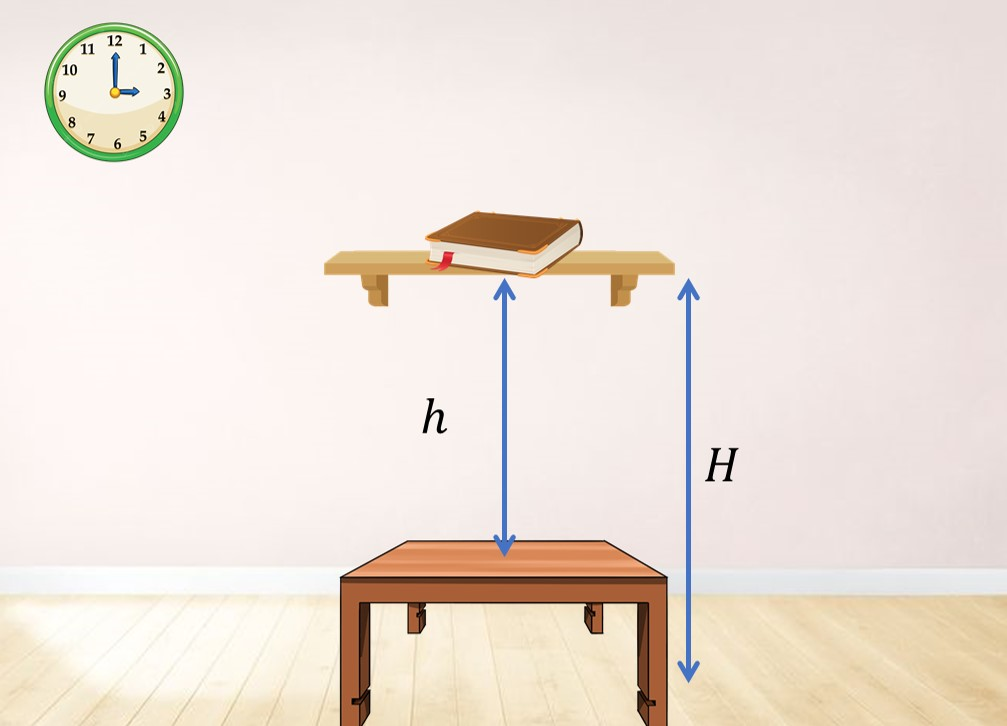
\includegraphics[width=0.4\linewidth]{../figs/VN10-2022-PH-TP026-P-2}
	\end{center}
	\choiceTF[t]
	{là sàn nhà thì thế năng của cuốn sách bằng $mgh$}
	{\True ở vị trí đặt cuốn sách thì thế năng bằng 0}
	{là mặt bàn thì thế năng của cuốn sách bằng $mg\left(H-h\right)$}
	{ở vị trí đồng hồ thì sách không có thế năng}
	\loigiai{}
\end{ex}
% ===================================================================
\begin{ex}\mkstar{2}
Một xe tải khối lượng 2 tấn đang chạy với tốc độ $\SI{72}{\kilo\meter/\hour}$ trên một đường thẳng nằm ngang theo chiều $xx'$ như hình thì đột ngột hãm phanh. Biết lực hãm được duy trì không đổi và bằng $\SI{12}{\kilo\newton}$.
\begin{center}
	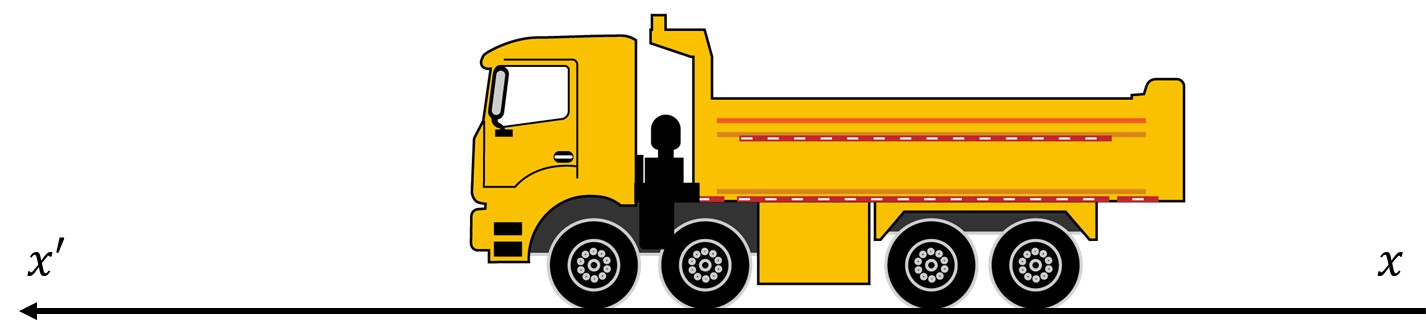
\includegraphics[width=0.5\linewidth]{../figs/VN10-2022-PH-TP026-P-3}
\end{center}
	\choiceTF[t]
	{\True Động năng của xe trước khi hãm phanh bằng $\SI{4E5}{\joule}$}
	{Lực hãm $\vec{F}_h$ tác dụng lên xe có chiều $xx'$}
	{\True Sau khi hãm phanh, xe có động năng giảm dần và thế năng không đổi}
	{\True Kể từ lúc hãm phanh cho đến khi dừng lại, xe đi được quãng đường $\xsi{\dfrac{100}{3}}{\meter}$}
	\loigiai{}
\end{ex}
% ===================================================================
\begin{ex}\mkstar{2}
	Người ta đẩy một cái thùng gỗ có khối lượng $\SI{55}{\kilogram}$ theo phương ngang với lực không đổi có độ lớn $\SI{220}{\newton}$ làm thùng bắt đầu chuyển động trên mặt phẳng ngang cùng hướng với lực tác dụng. Hệ số ma sát trượt giữa thùng và mặt phẳng là $\SI{0.35}{}$. Lấy $g =\SI{10}{\meter/\second^2}$.
	\choiceTF[t]
	{Thùng trượt đều trên sàn}
	{\True Công của lực đẩy khi thùng di chuyển được $\SI{1}{\meter}$ là $\SI{220}{\joule}$}
	{\True Công của lực ma sát trượt khi thùng di chuyển được $\SI{2}{\meter}$ là $\SI{-385}{\joule}$
	}
	{Sau khi di chuyển được $\SI{2}{\meter}$ kể từ thời điểm bắt đầu trượt, tốc độ của thùng là $\SI{2}{\meter/\second}$}
	\loigiai{
	\begin{itemchoice}
		\itemch Sai. Thùng trượt với gia tốc $a=\dfrac{F-\mu mg}{m}=\SI{0.5}{\meter/\second^2}$.
		\itemch Đúng.
		\itemch Đúng.
		\itemch Sai. $A_{F}-A_{F_{\mathrm{ms}}}=\dfrac{1}{2}mv^2\Rightarrow v=\xsi{\sqrt{2}}{\meter/\second}$.
	\end{itemchoice}
	}
\end{ex}

\Closesolutionfile{ans}
\section{Tự luận}
\setcounter{ex}{0}
\Opensolutionfile{ans}[ans/VN10-2022-PH-TP026-TL]
% ======================================================================
\begin{ex}\mkstar{2}
	Thả một quả bóng từ độ cao $h$ xuống sàn nhà. Động năng của quả bóng được chuyển hóa thành những dạng năng lượng nào ngay khi quả bóng chạm vào sàn nhà?
	\loigiai{Thả một quả bóng từ độ cao $h$ xuống sàn nhà. Ngay khi quả bóng chạm vào sàn nhà, chủ yếu động năng của quả bóng chuyển hóa thành thế năng làm quả bóng nảy lên, có một phần nhỏ động năng của quả bóng được chuyển hóa thành nhiệt năng (làm nóng quả bóng và mặt sàn) và năng lượng âm thanh (phát ra tiếng bụp ngay khi bóng chạm đất).}
\end{ex}
% ======================================================================
\begin{ex}\mkstar{2}
Khi đang bay, năng lượng của thiên thạch tồn tại dưới dạng nào? Tại sao năng lượng của thiên thạch lại rất lớn so với năng lượng của các vật thường gặp? Khi va vào Trái Đất, năng lượng của thiên thạch được chuyển hóa thành những dạng năng lượng nào?	
	\loigiai{
	\begin{itemize}
		\item Khi đang bay, năng lượng của thiên thạch tồn tại chủ yếu dưới dạng động năng và thế năng trọng trường, ngoài ra còn có quang năng, nhiệt năng.
		\item Năng lượng của thiên thạch rất lớn so với năng lượng của các vật thường gặp vì:
		\begin{itemize}
			\item Thiên thạch có khối lượng lớn.
			\item Thiên thạch di chuyển với tốc độ lớn $\Rightarrow$ có động năng lớn.
			\item Khoảng cách từ thiên thạch tới Trái Đất rất lớn $\Rightarrow$ có thế năng trọng trường rất lớn.
		\end{itemize}
		\item Khi va vào Trái Đất, năng lượng của thiên thạch được chuyển hóa thành động năng của các mảnh vỡ, tạo thành các hố lõm trên bề mặt Trái Đất.
	\end{itemize}
	}
\end{ex}
% ======================================================================
\begin{ex}\mkstar{2}
Một vận động viên quần vợt thực hiện cú giao bóng kỉ lục, quả bóng đạt tới tốc độ $\SI{196}{km/h}$. Biết khối lượng quả bóng là $\SI{60}{g}.$ Tính động năng của quả bóng.	
	\loigiai{Động năng của quả bóng được tính theo công thức:
		$$W_\text{đ} =\dfrac{1}{2}mv^2 \approx \SI{89}{J}.$$}
\end{ex}
% ======================================================================
\begin{ex}\mkstar{2}
	Máy đóng cọc có đầu búa nặng 0,5 tấn, được nâng lên độ cao $\SI{10}{m}$ so với mặt đất. Tính thế năng của đầu búa so với mặt đất. Lấy $g = \SI{9,8}{m/s}^2$.
	\loigiai{Thế năng của đầu búa
		$$W_\text{t} = mgh = \SI{49000}{J} = \SI{49}{kJ}.$$}
\end{ex}
% ======================================================================
\begin{ex}\mkstar{3}
	Một vật nhỏ $m$ được truyền vận tốc đầu $v_0=\SI{5}{m/s}$ tại A để vật trượt trên mặt phẳng ngang $\text{AB} = \SI{3}{m}$. Hệ số ma sát giữa vật và mặt ngang là $\mu=\SI{0.2}{}$. Lấy $g=\SI{10}{m/s^2}$. Tính vận tốc $v$ của vật tại B.
	\loigiai{Áp dụng định lý động năng:
		$$A_\text{ms} = \dfrac{1}{2}mv^2 - \dfrac{1}{2}mv_0^2 \Rightarrow -F_\text{ms}s = \dfrac{1}{2}mv^2 - \dfrac{1}{2}mv_0^2 \Rightarrow -\mu g s = \dfrac{1}{2}v^2 - \dfrac{1}{2}v_0^2 \Rightarrow v = \SI{3.6}{m/s}.$$}
\end{ex}
% ======================================================================
\begin{ex}\mkstar{3}
	Xe ô tô khối lượng 2 tấn bắt đầu khởi hành trên đường thẳng nằm ngang, đi được $\SI{50}{m}$ thì đạt được vận tốc $\SI{54}{km/h}$. Lực kéo của động cơ bằng $\SI{10000}{N}$. Lấy $g=\SI{10}{m/s^2}$.
	\begin{enumerate}[label=\alph*)]
		\item Dùng định lý động năng, tính công của lực ma sát.
		\item Tính độ lớn lực ma sát tác dụng lên xe trong đoạn đường trên.
	\end{enumerate}
	\loigiai{\begin{enumerate}[label=\alph*)]
			\item Dùng định lý động năng, tính công của lực ma sát.
			
			Áp dụng định lý động năng:
			$$A_F + A_\text{ms} = \dfrac{1}{2}mv^2 - 0 \Rightarrow A_\text{ms} = \dfrac{1}{2}mv^2 - A= \dfrac{1}{2} mv^2 - Fs= \SI{-275000}{J}.$$
			\item Tính độ lớn lực ma sát tác dụng lên xe trong đoạn đường trên.
			
			Ta có $A_\text{ms} = -F_\text{ms} s \Rightarrow F_\text{ms} = \SI{5500}{N}$.
	\end{enumerate}}
\end{ex}

% ======================================================================
\begin{ex}\mkstar{3}
		Một viên đạn có khối lượng $\SI{14}{g}$ bay theo phương ngang với vận tốc $\SI{400}{m/s}$ xuyên qua tấm gỗ dày $\SI{5}{cm}$, sau khi xuyên qua gỗ, đạn có vận tốc $\SI{120}{m/s}$. Tính lực cản trung bình của tấm gỗ tác dụng lên viên đạn.
	\loigiai{	Độ biến thiên động năng của viên đạn khi xuyên qua tấm gỗ là:
		$$\Delta W_\text{đ} = \dfrac{1}{2}mv^2_2 - \dfrac{1}{2}mv_1^2 = - \SI{1019.2}{\joule}.$$
		Theo định lí biến thiên động năng:
		$$A_\text{c} = \Delta W_\text{đ} = -F_\text{c}S \Rightarrow F_\text{c} = \SI{20384}{\newton}.$$}
\end{ex}
% ======================================================================
\begin{ex}\mkstar{3}
	Xe ô tô khối lượng 1 tấn bắt đầu khởi hành trên đường thẳng nằm ngang, đi được $\SI{50}{m}$ thì đạt được vận tốc $\SI{36}{km/h}$. Cho hệ số ma sát giữa bánh xe và mặt đường là $\SI{0.05}{}$. Lấy $g=\SI{10}{m/s^2}$. Dùng định lý động năng tính công của lực kéo của động cơ, từ đó suy ra độ lớn lực kéo của động cơ.
	\loigiai{Áp dụng định lý động năng:
		$$A_F + A_\text{ms} = \dfrac{1}{2}mv^2 - 0 \Rightarrow A_F = \dfrac{1}{2}mv^2 - A_\text{ms} = \dfrac{1}{2}mv^2 - (-F_\text{ms}s) = \SI{75000}{J}.$$
		Lực kéo của động cơ:
		$$A_F=Fs \Rightarrow F = \SI{1500}{N}.$$}
\end{ex}

	% ======================================================================
	\begin{ex}\mkstar{3}
		Một vật có khối lượng $m=\SI{2}{\kilogram}$ đang đứng yên thì bị tác dụng bởi lực $F$ và nó bắt đầu chuyển động thẳng. Độ lớn của lực $F$ và quãng đường $s$ mà vật đi được được biểu diễn trên đồ thị hình bên dưới.	
		\begin{center}
			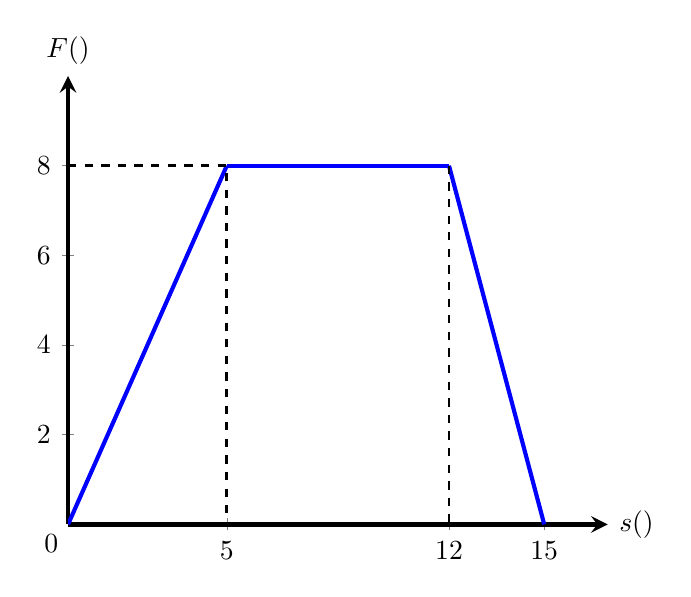
\begin{tikzpicture}  
				\begin{axis}[  ultra thick,
					xmin=0,  
					xmax=17,  
					xtick={0,5,12,15},
					ytick={0,2,...,8},
					ymin=0,  
					ymax=10, 
					samples=300,
					axis lines=center, 
					xlabel=$\xsi{s}{\left(\si{\meter}\right)}$, 		ylabel=$\xsi{F}{\left(\si{\newton}\right)}$,
					every axis y label/.style={at=(current axis.above origin),anchor=south},  
					every axis x label/.style={at=(current axis.right of origin),anchor=west},  ]
					\addplot [line width=1.5pt, blue, smooth, domain=0:5] {1.6*x};  
					\addplot [line width=1.5pt, blue, smooth, domain=5:12] {8}; 
					\addplot [line width=1.5pt, blue, smooth, domain=12:15] {8-8*(x-12)/3}; 
					\draw[dashed, line width=1pt] (axis cs: 0,8)--(axis cs:5,8)--(axis cs:5,0);
					\draw[dashed, line width=1pt] (axis cs:12,8)--(axis cs:12,0);
					\coordinate (O) at (axis cs: 0,0);
				\end{axis}  
				\node[below left] at (O) {0};
			\end{tikzpicture}
		\end{center}
		\begin{enumerate}[label=\alph*)]
			\item Tính công của lực $\vec{F}$.
			\item Tìm vận tốc của vật tại vị trí ứng với điểm cuối của đồ thị.
		\end{enumerate}
		\loigiai{
			\begin{enumerate}[label=\alph*)]
				\item $A=\SI{88}{\joule}$.
				\item $v=\sqrt{\dfrac{2A}{m}}\approx\SI{9.38}{\meter/\second}$.
			\end{enumerate}
		}
	\end{ex}
	% ======================================================================
	\begin{ex}\mkstar{3}
		Một ô tô có khối lượng $m=\SI{1.20}{\text{tấn}}$ chuyển động lên trên một con dốc phẳng có độ dài $s=\SI{1.50}{\kilo\meter}$ với vận tốc $v=\SI{54.0}{\kilo\meter/\hour}$. Chiều cao của đỉnh dốc so với mặt phẳng nằm ngang đi qua chân dốc (gốc thế năng nằm ở chân dốc) là $h=\SI{30.0}{\meter}$.
		Biết gia tốc rơi tự do là $g=\SI{9.8}{\meter/\second^2}$.
		\begin{enumerate}[label=\alph*)]
			\item Tính thế năng của ô tô ở đỉnh con dốc.
			\item Lấy gốc thời gian là lúc ô tô ở chân dốc, tìm thời điểm thế năng của ô tô bằng $\varepsilon=\SI{25}{\percent}$ thế năng của nó tại đỉnh dốc.
			\item Xác định công suất của động cơ ô tô biết rằng tỉ số giữa thế năng của ô tô với công mà động cơ của nó thực hiện là $\eta=\SI{90.0}{\percent}$.
		\end{enumerate}
		\loigiai{
		\begin{enumerate}[label=\alph*)]
			\item Thế năng của ô tô khi nó ở đỉnh dốc:
			$$W_{\text{th}}=mgh\approx\SI{353}{\kilo\joule}.$$
			\item Ta có:
			$$\dfrac{W_{\text{t}}}{W_{\text{th}}}=\dfrac{mgh_{\text{t}}}{mgh}=\dfrac{h_{\text{t}}}{h}=\dfrac{s_{\text{t}}}{s_{\text{h}}}=\dfrac{vt}{s}=\varepsilon$$
			Trong đó $h_{\text{t}}$ là độ cao của ô tô (so với chân dốc) ở thời điểm $t$, $s_{\text{t}}$ là quãng đường ô tô đi được trong khoảng thời gian $t=\dfrac{\varepsilon s}{v}=\SI{25.0}{\second}$.
			\item Ta có:
			$$\eta=\dfrac{W_{\text{t}}}{A}=\dfrac{mgh_{\text{t}}}{\calP t}$$
			Từ câu b, ta có:
			$$h_{\text{t}}=\dfrac{hvt}{s}\Rightarrow \eta=\dfrac{mg}{\calP t}\cdot\dfrac{hvt}{s}=\dfrac{mghv}{\calP s}.$$
			Công suất của động cơ ô tô:
			$$\calP=\dfrac{mghv}{\eta s}=\SI{3.92}{\kilo\watt}.$$
		\end{enumerate}
		}
	\end{ex}
% ======================================================================
\begin{ex}\mkstar{3}
Một vật có khối lượng $m=\SI{1.00}{\kilogram}$ được thả rơi không vận tốc đầu từ độ cao $h=\SI{10.0}{\meter}$ so với mặt đất. Vật dừng lại sau khi ngập sâu vào lòng đất đoạn $d=\SI{30.0}{\centi\meter}$ theo phương thẳng đứng. Biết rằng gia tốc rơi tự do là $g=\SI{9.80}{\meter/\second^2}$. Lấy gốc thế năng là mặt đất. Tính:
\begin{enumerate}[label=\alph*)]
	\item thế năng cực tiểu của vật trong quá trình chuyển động;
	\item công mà mặt đất truyền cho vật.
\end{enumerate}	
	\loigiai{
	\begin{enumerate}[label=\alph*)]
		\item Thế năng của vật đạt giá trị cực tiểu khi nó ở độ sâu cực đại:
		$$W_{\text{t min}}=-mgd=\SI{-2.94}{\joule}.$$
		\item Công mà mặt đất truyền cho vật, áp dụng định lý động năng:
		$$0-\dfrac{1}{2}mv^2=A_{\vec{P}}+A_{\vec{F}_c}\Rightarrow A_{\vec{F}_c}=-\dfrac{1}{2}mv^2-A_{\vec{P}}$$
		$$\Rightarrow A_{\vec{F}_c}=-mgh-mgd=-mg(h+d)\approx\SI{-101}{\joule}.$$
	\end{enumerate}
	}
\end{ex}
\Closesolutionfile{ans}